% !Mode:: "TeX:UTF-8"

\chapter{}
\textbf{
Suppose that we are given a weighted, directed graph $G=(V,E)$ in which edges that leave the source vertex $s$ may have negative weights, all other edge weights are nonnegative, and there are no negative-weight cycles. Argue that Dijkstra's algorithm correctly finds shortest paths from $s$ in this graph.
}

Because only those edges that leave the source vertex $s$ may have negative weights, so the triangle inequality in the proof of traditional Dijkstra's algorithm is still correct.
\begin{figure}[!htbp]
\centering
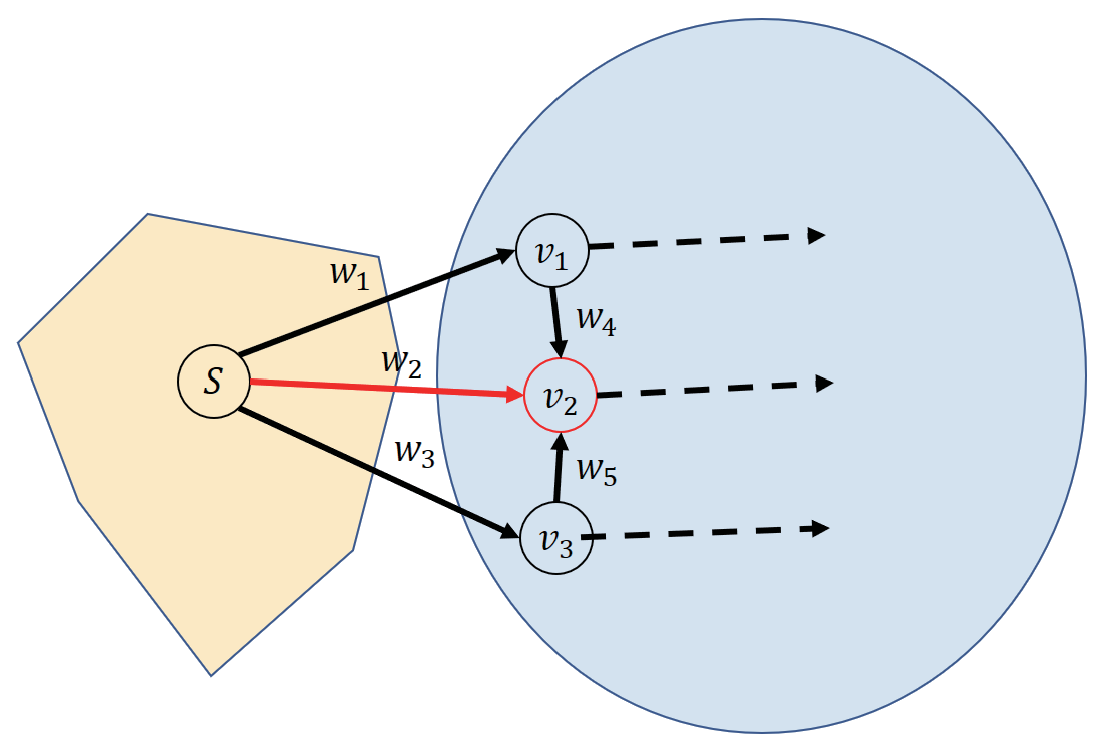
\includegraphics[width=0.5\textwidth]{figures/2.eps}
\caption{Only edges that leave the source vertex $s$ may have negative weights}\label{fig_2_1}
\end{figure}
 As shown in Fig~\ref{fig_2_1}, suppose $v_2$ is the first chosen vertex, then we have $w_2\leq w_1$ and $w_2\leq w_3$. No matter is $w_2$ positive or negative, we always have $w_1+w_4\geq w_2+w_4\geq w_2$(because $w_4$ is positive). Therefore, Dijkstra's algorithm correctly finds shortest paths from $s$ in this graph.
